\documentclass{article}
\usepackage{graphicx}
\usepackage{tikz}
\usepackage{amsmath}
\usepackage{hyperref}
\usepackage[a4paper, margin=2.5cm]{geometry}
\setlength{\parindent}{0pt} % Set paragraph indentation to zero

\begin{document}

\section*{Neuron}

Schema of a neuron:
\begin{center}
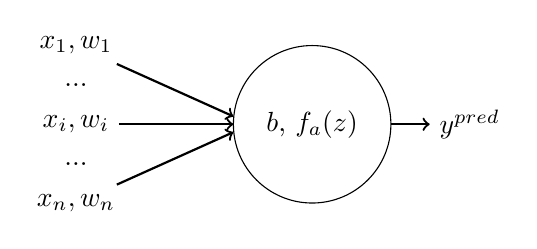
\begin{tikzpicture}
  % Draw a circle with radius 1
  \draw (3,2) circle (1);
  \node[black] at (3,2) {$b$, $f_a(z)$};
  \node[black] (x1) at (0,3) {$x_1, w_1$};
  \draw[->, thick] (x1) -- (2,2.1);
  \node[black] at (0,2.5) {...};
  \node[black] (xi) at (0,2) {$x_i, w_i$};
  \draw[->, thick] (xi) -- (2,2);
  \node[black] at (0,1.5) {...};
  \node[black] (xn) at (0,1) {$x_n, w_n$};
  \draw[->, thick] (xn) -- (2,1.9);
  \node[black] (out) at (5,2) {$y^{pred}$};
  \draw[->, thick] (4,2) -- (out);
\end{tikzpicture}
\end{center}

To compute predicted value by the neuron:
\begin{equation}
  z = \sum_{i=1}^n w_ix_i + b
\end{equation}

\begin{equation}
  y^{pred} = f_a(z) = f_a(\sum_{i=1}^n w_ix_i + b)
\end{equation}

To compute the cost function for $m$ training samples:
\begin{align}
  C(w,b) &= \frac{1}{2m} \sum_{j=1}^m \left(y_j^{pred} - y_j\right)^2 \nonumber \\
         &= \frac{1}{2m} \sum_{j=1}^m \left(f_a(z)_j - y_j\right)^2
\end{align}

Training the neuron consists on minimizing the cost function. The method used to minimize the cost function is Gradient Descent (\url{https://en.wikipedia.org/wiki/Gradient_descent}).

\begin{align}
  \mathbf{w}^{n+1} &= \mathbf{w}^n - \alpha \nabla C(\mathbf{w}^n, b^n) \\
  b^{n+1} &= b^n - \alpha \nabla C(\mathbf{w}^n, b^n)
\end{align}

The equations above compute the gradient descent for the weights and for the bias. $\alpha$ is the so called Learning Rate.

To compute the gradient of the cost function for $m$ training samples, it is necessary to compute the partial derivatives with respect $\mathbf{w}$ and $b$.

Partial derivative with respect $\mathbf{w}$:
\begin{align}
  \dfrac{\delta C(\mathbf{w},b)}{\delta w_i}
  &= \left( \frac{1}{2m} \left(f_a(z) - y\right)^2 \right)' \nonumber \\
  &= \frac{1}{m} \left(f_a(z) - y\right) f_a'(z) z' \nonumber \\
  &= \frac{1}{m} \sum_{j=1}^m \left(f_a(\mathbf{w \cdot x} + b) - y_j\right) f_a'(\mathbf{w \cdot x} + b) (x_i)_j
\end{align}

In a similar way, the partial derivative with respect $b$:
\begin{equation}
  \dfrac{\delta C(\mathbf{w},b)}{\delta b} = \frac{1}{m} \sum_{j=1}^m \left(f_a(\mathbf{w \cdot x} + b) - y_j\right) f_a'(\mathbf{w \cdot x} + b)
\end{equation}

\section*{Activation functions}

\subsection*{Sigmoid}

Sigmoid function is:
\begin{equation}
  \sigma(x) = \frac{1}{1 + e^{-x}}
\end{equation}

Sigmoid derivative is:
\begin{equation}
  \sigma'(x) = \sigma(x) \cdot (1 - \sigma(x))  
\end{equation}

\subsection*{ReLU}

ReLU function is:
\begin{equation}
  ReLU(x) = \max(0,x)
\end{equation}

The derivative of the ReLU function is:
\begin{equation}
  ReLU'(x) = \begin{cases} 
    0 & x < 0 \\
    1 & x\geq 0 
  \end{cases}
\end{equation}

\end{document}
